\chapter{Aplikace a~ukázková hra}
V~této části popíšeme instalaci aplikace, použití grafického rozhraní a~uvedeme návod pro hraní ukázkové hry. 

\section{Instalace}
Pro instalaci platformy spusťte soubor \texttt{setup.exe}, umístěný v~přílohách práce \ref{sec:appendix}. Po spuštění instalátoru budete vyzváni k~výběru umístění aplikace. Platforma vyžaduje instalaci do adresáře, ve kterém má každý uživatel spouštějící platformu možnost zápisu. Následně bude aplikace nainstalována spolu se všemi svými závislostmi. V~aktuální verzi je jedinou závislostí platformy Microsoft .NET Framework 4.7.2 (x86 and x64).

\section{Grafické rozhraní}
Grafické uživatelské rozhraní platformy je tvořeno několika obrazovkami, které můžeme vidět na diagramu \ref{fig:screen_structure2}. Přechody mezi obrazovkami jsou iniciovány za použití grafických prvků těchto obrazovek, či jsou řízeny průběhem akce na pozadí. V~této části popíšeme použití složitějších obrazovek uživatelského rozhraní.

\begin{figure}[h]
	\centering
	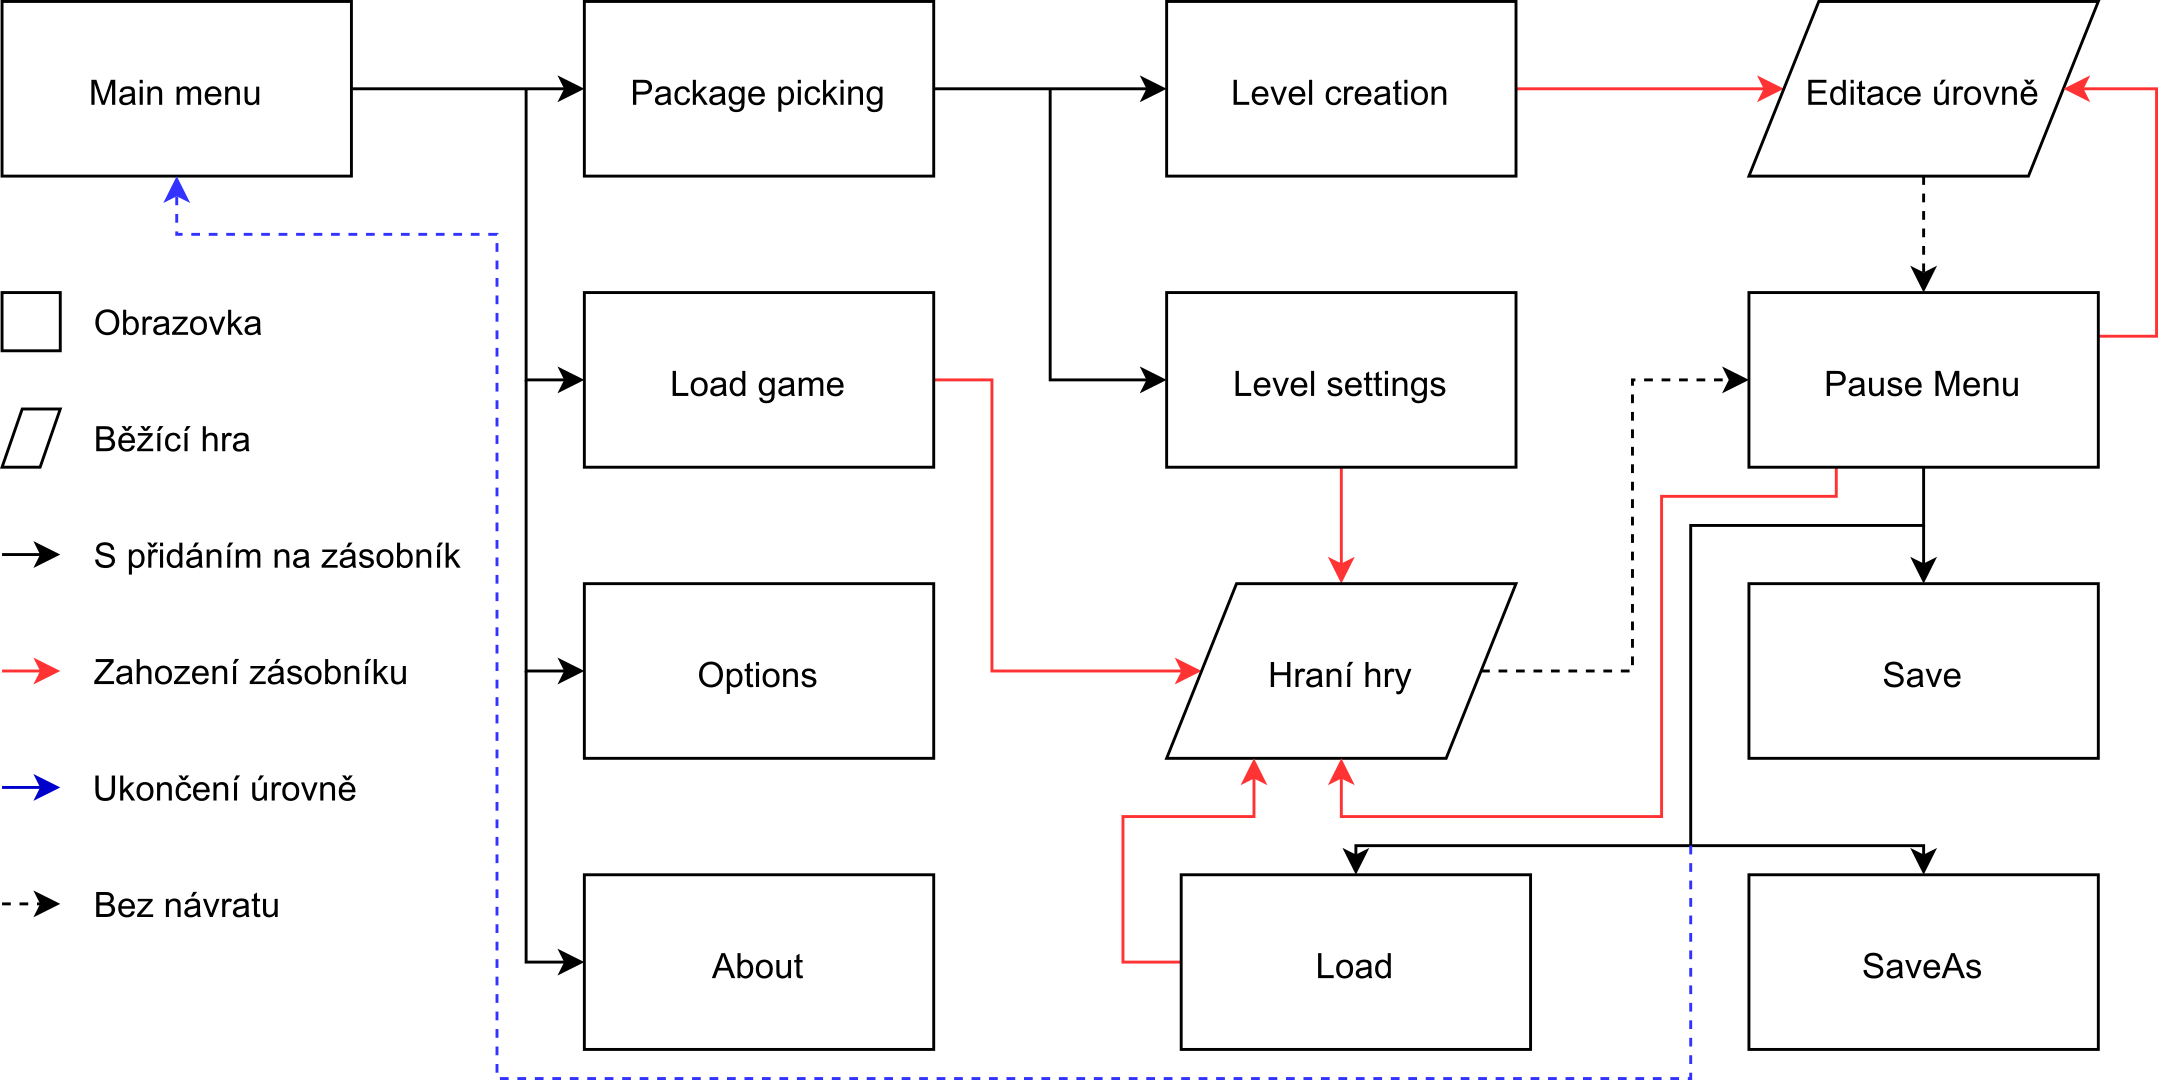
\includegraphics[width=\textwidth]{img/ScreenStructure.png}
	\caption{Obrazovky menu a~přechody mezi nimi.}
	\label{fig:screen_structure2}
\end{figure}

\subsection{Výběr balíčků}
Obrazovka pro výběr balíčků, na diagramu \ref{fig:screen_structure2} označena \texttt{Package picking}, je z~hlavního menu přístupná stisknutím tlačítka \texttt{Start}. Obrazovku můžeme vidět na obrázku \ref{fig:packagepicking}. Centrální část obrazovky zabírá seznam balíčků dostupných v~aktuální instalaci platformy. Každý z~balíčků je reprezentován jednou položkou tohoto seznamu. 

\begin{figure}[h]
	\centering
	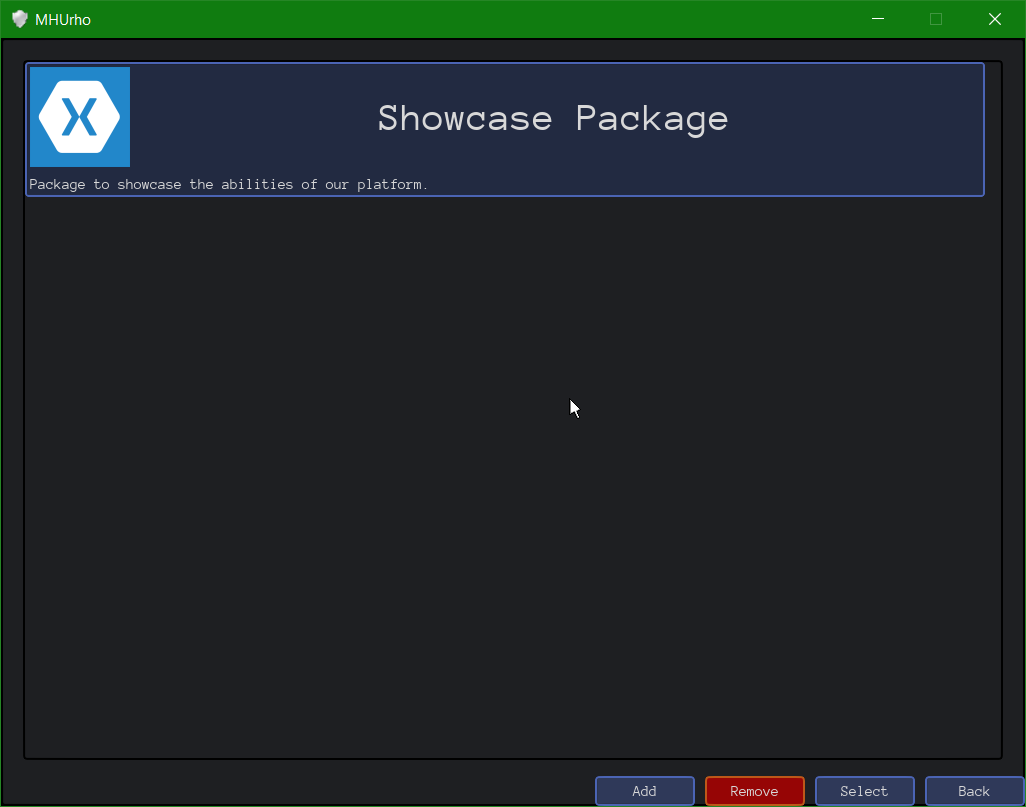
\includegraphics[width=0.5\textwidth]{img/PackagePickingScreen.png}
	\caption{Obrazovky pro výběr balíčku.}
	\label{fig:packagepicking}
\end{figure}

Pro přidání nového balíčků do nainstalované instance platformy přemístěte adresář obsahující soubory balíčku do adresáře \texttt{\%AppData\%/MHUrho/Packages}. Následně stiskněte tlačítko \texttt{Add}, neboli \uv{Přidat}, na obrazovce pro vybírání balíčků. Toto tlačítko vás přesune na obrazovku pro procházení souborového systému. Na této obrazovce poté vyberte XML soubor definující přidávaný balíček. Při návratu na obrazovku pro vybírání balíčků by měl být přidaný balíček viditelný v~seznamu dostupných balíčků. d

Pro smazání balíčku označte položku balíčku v~seznamu a~stiskněte tlačítko \texttt{Remove}. Pro načtení balíčku  označte položku balíčku a~stisknute tlačítko \texttt{Select}. Pro návrat na obrazovku hlavního menu použijte tlačítko \texttt{Back}.

\subsection{Výběr úrovně}
Po vybrání balíčku budete přesunuti na obrazovku výběru úrovně, v~diagramu označenou jako \texttt{Level picking}. Tuto obrazovku můžete vidět na obrázku \ref{fig:levelpicking}. Tato obrazovka poskytuje následující funkce:

\begin{enumerate}
	\item vytváření a~editaci nových úrovní,
	\item editaci existujících úrovní,
	\item spuštění existujících úrovní,
	\item mazání úrovní v~balíčku.
\end{enumerate}

Pro vytvoření nové úrovně označte položku \texttt{Create new level} a~následně stiskněte tlačítko \texttt{Edit}.

\begin{figure}[h]
	\centering
	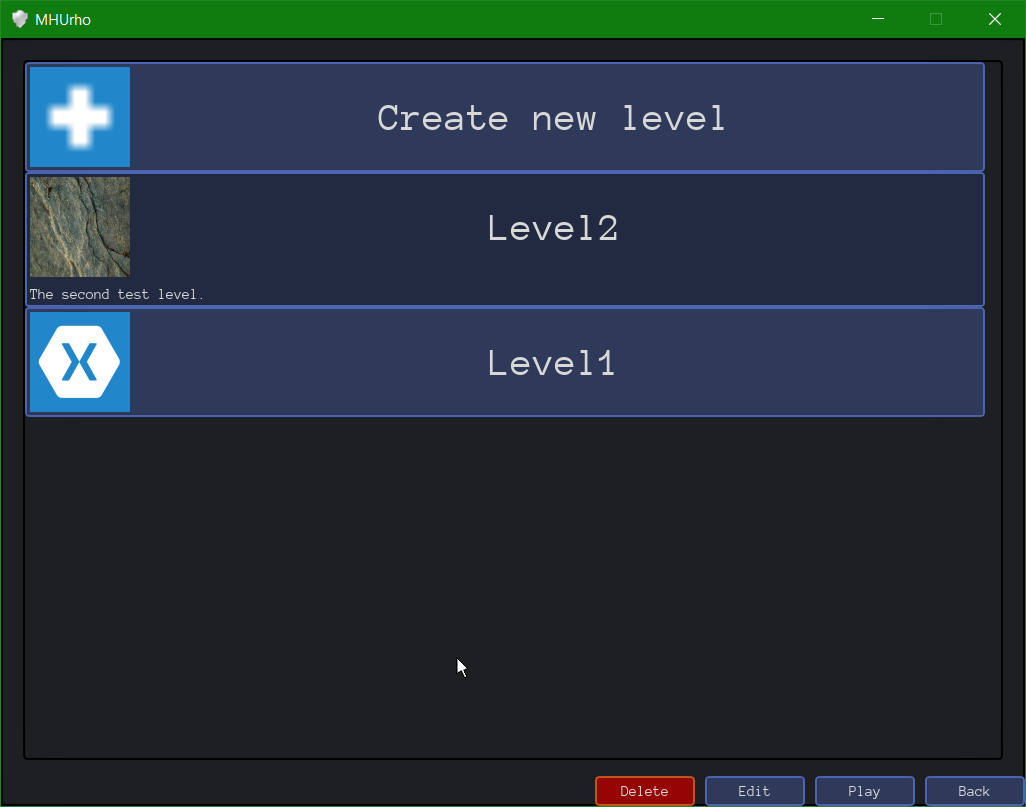
\includegraphics[width=0.5\textwidth]{img/LevelPickingScreen.png}
	\caption{Obrazovky pro výběr úrovně.}
	\label{fig:levelpicking}
\end{figure}

Pro akci s~existující úrovní označte tuto úroveň v~seznamu. Následně stisknutím tlačítka \texttt{Delete} smažete úroveň, stisknutím tlačítka \texttt{Edit} přejdete na obrazovku \texttt{Level creation} a~následně na editaci úrovně a~stisknutím tlačítka \texttt{Play} přejdete na obrazovku \texttt{Level settings} pro nastavení parametrů spuštění úrovně.

Pro návrat na obrazovku výběru balíčků použijte tlačítko \texttt{Back}.
\subsection{Vytváření úrovně}
Při vytváření úrovně či editaci existující úrovně budete přesunuti na obrazovku označenou v~diagramu \ref{fig:screen_structure2} jako \texttt{Level creation}. Vzhled této obrazovky můžete vidět na obrázku \ref{fig:levelcreation}. Jak můžete vidět, tato obrazovka umožňuje nastavit tyto vlastnosti úrovně:

\begin{enumerate}
	\item jméno,
	\item velikost mapy,
	\item plugin logiky,
	\item ikonu,
	\item popis.
\end{enumerate}

Při editaci existující úrovně nelze měnit její velikost a~plugin logiky.

\begin{figure}[h]
	\centering
	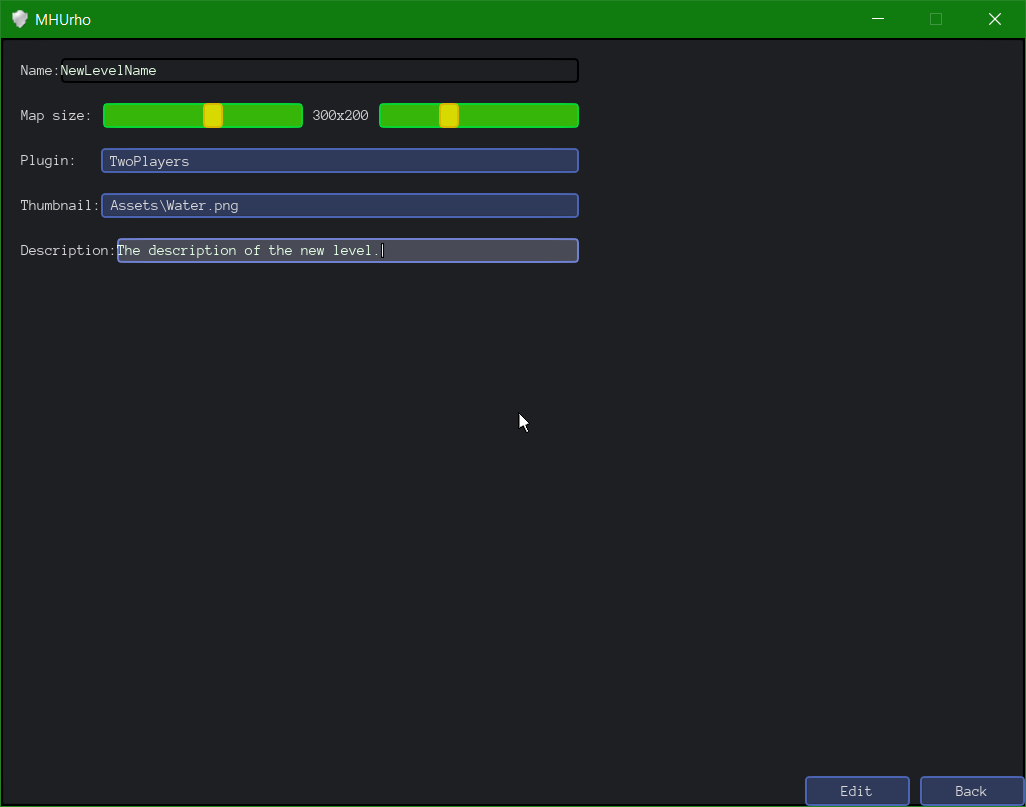
\includegraphics[width=0.5\textwidth]{img/LevelCreationScreen.png}
	\caption{Obrazovky pro nastavení vlastností vytvářené úrovně.}
	\label{fig:levelcreation}
\end{figure}

Pro návrat na obrazovku výběru úrovní použijte tlačítko \texttt{Back}.

\subsection{Nastavení úrovně}
Pro nastavení vlastností úrovně před samotným spuštěním slouží obrazovka \texttt{Level settings}, zobrazená na obrázku \ref{fig:levelsettings}. Obrazovka je rozdělena do čtyř částí:

\begin{enumerate}
	\item výběr pluginu hráčů úrovně a~nastavení jejich příslušenství do týmu;
	\item zobrazení ikony úrovně;
	\item zobrazení prvků grafického uživatelského rozhraní definovaných pluginem úrovně, používaných pro nastavení parametrů spouštěné úrovně;
	\item zobrazení popisu úrovně.
\end{enumerate}

Stisknutím tlačítka \texttt{Play} je spuštěno načítání úrovně a~následně hra. Stisknutím tlačítka \texttt{Back} dojde k~přesunu zpět na obrazovku vybírání úrovní.

\begin{figure}[h]
	\centering
	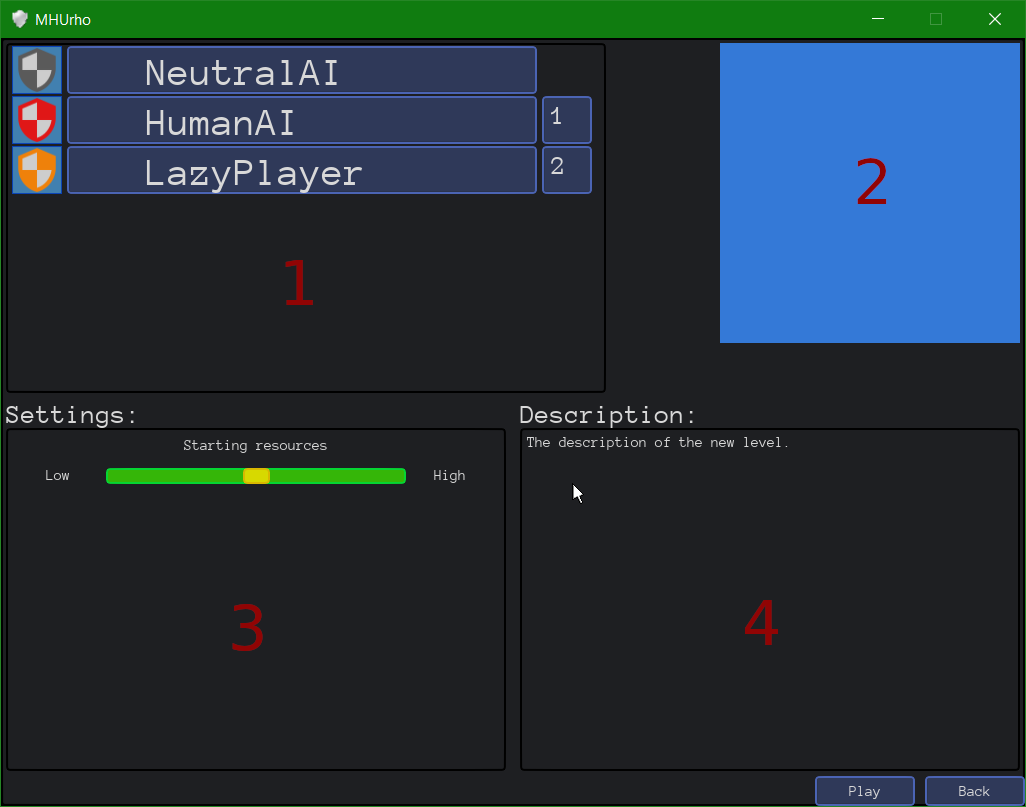
\includegraphics[width=0.5\textwidth]{img/LevelSettingsScreen.png}
	\caption{Obrazovky pro nastavení spuštěné hry.}
	\label{fig:levelsettings}
\end{figure}

\subsection{Přerušení hry}
Při pozastavení hry je zobrazeno tzv.~\texttt{PauseMenu}. Položky tohoto menu se liší podle toho, zda úroveň editujeme či úroveň hrajeme. Porovnání těchto dvou menu můžeme vidět na obrázku \ref{fig:pauseMenu}.

Při editaci umožňuje menu uložit aktuální stav úrovně do balíčkupod jménem nastaveným při vytváření úrovně pomocí tlačítka \texttt{Save} či pod novým jménem pomocí tlačítka \texttt{SaveAs}.

Při hraní hry umožňuje menu uložit aktuální stav hrané hry do adresáře platformy pomocí tlačítka \texttt{Save}, či načíst hranou hru uloženou v~tomto adresáři pomocí tlačítka \texttt{Load}.

\begin{figure}[h]
	\centering
	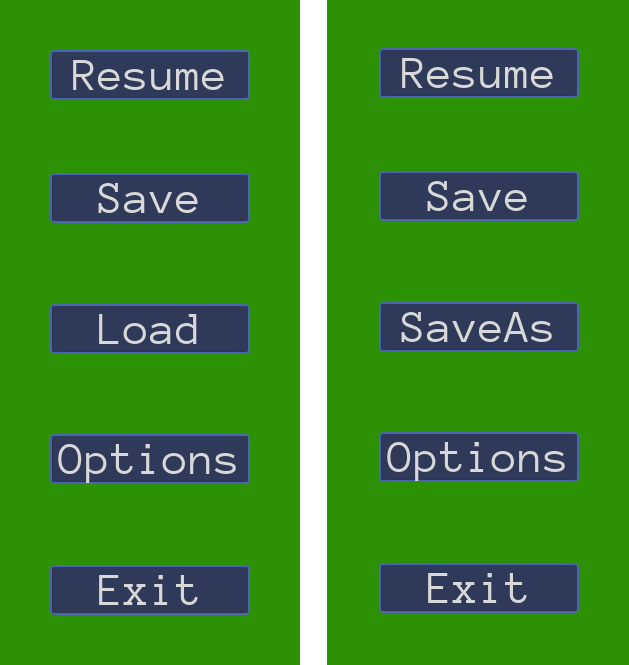
\includegraphics[width=0.5\textwidth]{img/PauseMenuComparison.png}
	\caption{Menu pozastavení hry.}
	\label{fig:pauseMenu}
\end{figure}


\subsection{Výběr souboru}
Obrazovku pro výběr souboru můžeme vidět na obrázku \ref{fig:filepicking}. Modře označená část výpisu obsahu adresáře představuje podadresáře, bílá část pak soubory. V~horní části můžeme vidět vyhledávací řádek, do kterého je možno napsat část jména pro filtrování zobrazených souborů či přímo celou cestu vybíraného souboru či adresáře. Pro výběr lze použít tlačítko \texttt{Select}, které vybere soubor či adresář podle cesty ve vyhledávacím řádku, či dvojklikem na záznam vybíraného souboru.

Obrazovky pro ukládání a~načítání hraných úrovní z~adresáře platformy poskytují navíc tlačítko \texttt{Delete}, kterým je možné uloženou hru smazat.

\begin{figure}[h]
	\centering
	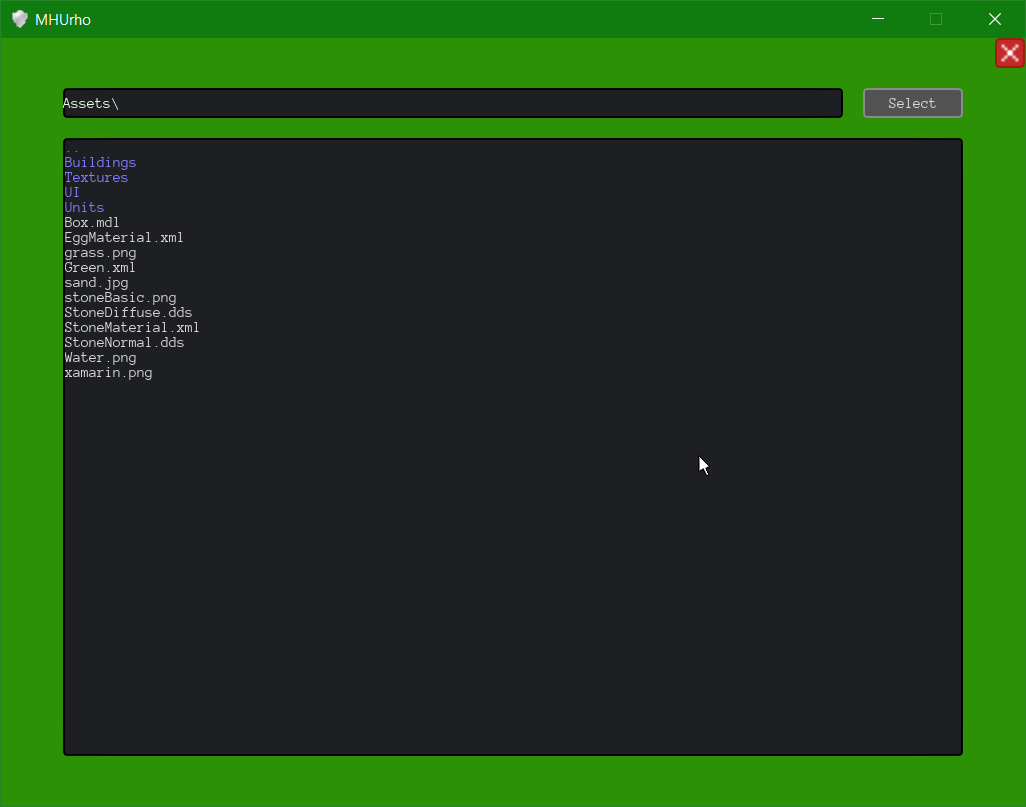
\includegraphics[width=0.5\textwidth]{img/FilePickingScreen.png}
	\caption{Obrazovka pro výběr souboru.}
	\label{fig:filepicking}
\end{figure}

\section{Ukázková hra}
Ukázková hra je reprezentována balíčkem \texttt{ShowcasePackage}. Tento balíček obsahuje jednotky, budovy, projektily a~další součásti hry, které je možné využít pro tvorbu úrovní. Současně obsahuje několik již vytvořených úrovní demonstrujících schopnosti protihráčů, jednotek a~budov.

\subsection{Okno aplikace při hře}
\label{sec:appwindow}
Okno aplikace má při hře platformou definované základní uživatelské rozhraní. Toto rozhraní můžeme vidět na obrázku \ref{fig:UI}. 

Minimapa poskytuje hráči přehled o~stavu velké části mapy bez nutnosti pohybu kamerou. Minimapu lze přibližovat či oddalovat za použití kolečka myši při umístění kurzoru nad minimapu. Dále lze kliknutím přesunout kameru na odpovídající pozici v~herním světě. V~neposlední řadě lze minimapu použít k~rychlému přesunu kamery pomocí kliknutí a~držení levého tlačítka a~posunu myší. Pozice kliknutí se stává středem pomyslného joysticku, který ovládáme posunem myši odpovídajícím směrem.

Centrální lišta obsahuje tlačítka určená aktuálně zvoleným nástrojem. Při velkém počtu tlačítek je možno touto lištou posouvat za použití tlačítek označených šipkami na pravé a~levé straně lišty.

Nad lištou vidíme vpravo tlačítko pro výběr aktuálního hráče a~vlevo tlačítko pro výběr nástroje. Výběr hráče je možný pouze při editaci úrovně. Při hraní je toto tlačítko neaktivní a~pouze zobrazuje ikonu hráče reprezentujícího uživatele. Tlačítko pro výběr budovy, stejně jako tlačítko pro výběr hráče při editaci, při kliknutí zobrazí vysouvací lištu, označenou fialově. Tato lišta obsahuje seznam dostupných nástrojů či seznam dostupných hráčů.

Poslední součástí v~levém dolním rohu je \texttt{CustomWindow}. Obsah této části je určen aktuálním nástrojem. Nejčastěji je v~této části uváděn název nástroje či součásti nástroje, nastavní velikosti štětce, cena budov a~další.

Balíček může do uživatelského rozhraní dodat vlastní prvky, jak můžeme vidět ve vrchní části obrazovky, ve které balíček ukázkové hry umisťuje lištu pro zobrazení množství surovin vlastněných hráčem.

\begin{figure}[h]
	\centering
	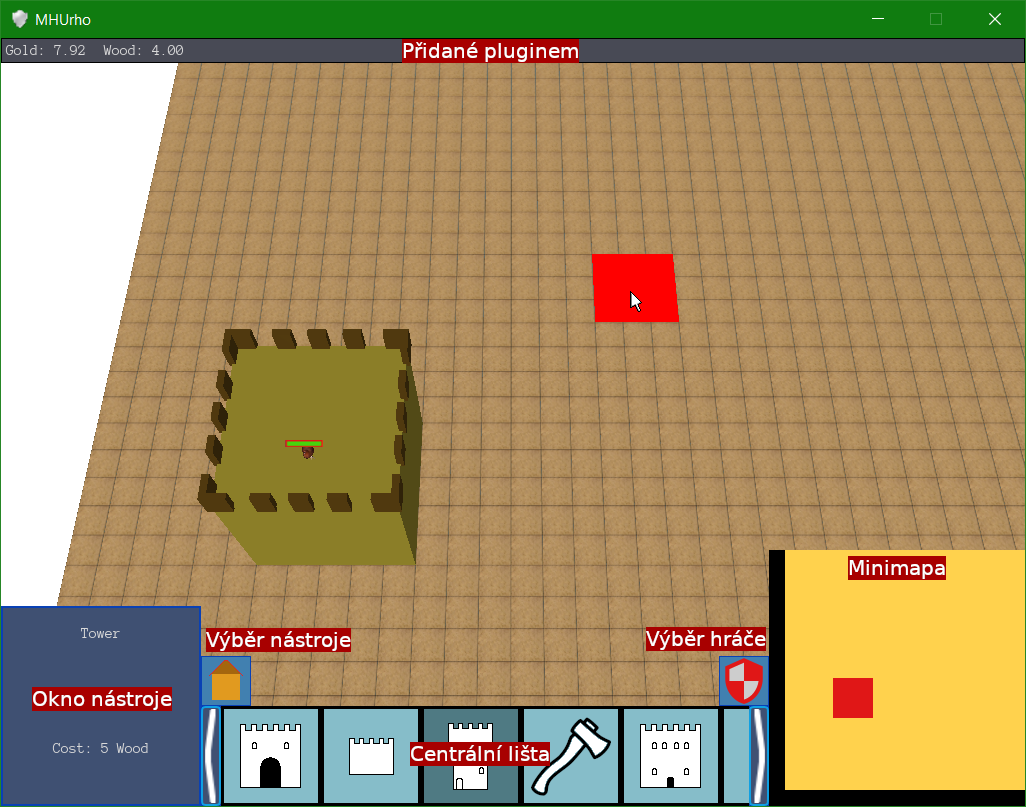
\includegraphics[width=0.5\textwidth]{img/GameUI.png}
	\caption{Uživatelské rozhraní ukázkové hry.}
	\label{fig:UI}
\end{figure}

\subsection{Editor}
Každý z~balíčků, tedy i~ukázková hra, může použít nástroje poskytované platformou či definovat své vlastní nástroje pro editaci úrovně. V~této části popíšeme použití nástrojů dostupných v~editoru úrovní ukázkové hry.

\subsubsection{Nástroje}

Výběr nástroje lze provést stisknutím tlačítka označeného na obrázku \ref{fig:UI} jako \textit{Výběr nástroje}. Stisknutím tohoto tlačítka je zobrazena lišta se seznamem všech dostupných nástrojů, kterou můžete vidět na obrázku \ref{fig:toolselection}. V této liště můžeme vidět označený aktuálně vybraný nástroj, jehož vzhled přebírá také tlačítko pro výběr nástroje. 

Stisknutím tlačítka jiného nástroje než aktuálně vybraného je tento nástroj aktivován a je schována lišta pro výběr nástrojů.

Následuje seznam nástrojů dostupných v ukázkové hře. U každého z nástrojů je uvedeno, ve kterých módech je možné ho využít. Bližší popis jednotlivých nástrojů můžete najít následujících částech.

\medskip
\noindent{
	\begin{minipage}{0.15\textwidth}
		
\includegraphics{TerrainManipulatorTool}
	\end{minipage} \hfill
	\begin{minipage}{0.8\textwidth}
		\textbf{Nástroj pro změnu výšky terénu} umožňuje změnu výšky jednotlivých rohů dlaždic, celých dlaždic uvnitř čtverce či vyhlazení rozdílů ve výšce dlaždic uvnitř čtverce. Tento nástroj je dostupný pouze v editačním módu.
	\end{minipage}	
}

\medskip
\noindent{
	\begin{minipage}{0.15\textwidth}
		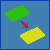
\includegraphics{TileTypeTool}
	\end{minipage} \hfill
	\begin{minipage}{0.8\textwidth}
		\textbf{Nástroj pro změnu typů dlaždic} umožňuje změnu typu dlaždic. Tento nástroj je dostupný pouze v editačním módu.
	\end{minipage}
}

\medskip
\noindent{
	\begin{minipage}{0.15\textwidth}
		
\includegraphics{UnitSelectorTool}
	\end{minipage} \hfill
	\begin{minipage}{0.8\textwidth}
		\textbf{Nástroj pro výběr a ovládání jednotek} umožňuje označit vybrat skupinu jednotek a následně této skupině vydávat rozkazy pro pohyb či pro útok. Tento nástroje je dostupný v editačním i herním módu.
	\end{minipage}
}

\medskip
\noindent{
	\begin{minipage}{0.15\textwidth}
		
\includegraphics{UnitSpawningTool}
	\end{minipage} \hfill
	\begin{minipage}{0.8\textwidth}
		\textbf{Nástroj pro vytváření jednotek} umožňuje přidat do úrovně jednotky vlastněné aktuálně ovládaným hráčem. Tento nástroje je dostupný pouze v editačním módu.
	\end{minipage}
}

\medskip
\noindent{
	\begin{minipage}{0.15\textwidth}
		
\includegraphics{BuildingBuilderTool}
	\end{minipage} \hfill
	\begin{minipage}{0.8\textwidth}
		\textbf{Nástroj pro stavbu budov} umožňuje přidat do úrovně budovy vlastněné aktuálně ovládaným hráčem. Tento nástroje je dostupný v editačním i herním módu.
	\end{minipage}
}

\subsubsection{Nástroj pro změnu výšky terénu}
Tento nástroj umožňuje měnit reliéf terénu aktuální úrovně. Nástroj je složen ze čtyř součástí. Těmito součástmi jsou:

\medskip
\noindent{
	\begin{minipage}{0.15\textwidth}
		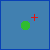
\includegraphics{VertexSelection}
	\end{minipage} \hfill
	\begin{minipage}{0.8\textwidth}
		Výběr rohů dlaždic.
	\end{minipage}
}

\medskip
\noindent{
	\begin{minipage}{0.15\textwidth}
		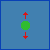
\includegraphics{VertexMovement}
	\end{minipage} \hfill
	\begin{minipage}{0.8\textwidth}
		Změny výšky vybraných rohů dlaždic.
	\end{minipage}
}

\medskip
\noindent{
	\begin{minipage}{0.15\textwidth}
		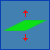
\includegraphics{TileMovement}
	\end{minipage} \hfill
	\begin{minipage}{0.8\textwidth}
		Změna výšky dlaždic uvnitř zvýrazněného čtverce.
	\end{minipage}
}

\medskip
\noindent{
	\begin{minipage}{0.15\textwidth}
		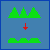
\includegraphics{Smoothing}
	\end{minipage} \hfill
	\begin{minipage}{0.8\textwidth}
		Vyhlazen rozdílů výšky dlaždic uvnitř zvýrazněného čtverce.
	\end{minipage}
}
\bigskip


První dvě součásti jsou dohromady používány pro výběr jednotlivých rohů dlaždic v mapě a následnou úpravu jejich výšky. Výběr lze provést zvolením části pro výběr rohů a následným kliknutím na dlaždici obsahující daný roh. Je vybrán roh nejbližší pozici kliknutí. Zrušení výběru lze následně provést pokusem o výběr již vybraného rohu. Pro změnu výšky vybraných rohů zvolíme část pro změnu výšky vybraných rohů. Po jejím zvolení můžeme kliknutím a držením levého tlačítka a posouváním myši nahoru a dolu měnit výšku vybraných rohů.

Součást pro změnu výšky dlaždic umožňuje pohybem kurzoru po herním světě vybrat čtverec dlaždic okolo pozice kurzoru, jejichž výšku měníme pomocí stisknutí a držení levého tlačítka a pohybem myši stejně jako u předchozí části.

Poslední součást pro vyhlazení terénu umožňuje stisknutím a držením levého tlačítka myši a pohybem po mapě vyrovnávat rozdíly výšky terénu.

\subsubsection{Nástroj pro změnu typu dlaždic}
Při zvolení tohoto nástroje je centrální lišta vyplněna všemi dostupnými typy dlaždic v balíčku. V ukázkovém balíčku bude centrální lišta vyplněna těmito ikonami:

\medskip
\noindent{
	\begin{minipage}{0.1\textwidth}
		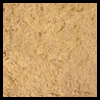
\includegraphics[scale=0.3]{SandIcon}
	\end{minipage} \hfill
	\begin{minipage}{0.85\textwidth}
		Ikona typu dlaždic \texttt{Sand}, neboli písek.
	\end{minipage}
}

\medskip
\noindent{
	\begin{minipage}{0.1\textwidth}
		
\includegraphics[scale=0.3]{XamarinIcon}
	\end{minipage} \hfill
	\begin{minipage}{0.85\textwidth}
		Ikona typu dlaždic \texttt{Xamarin}.
	\end{minipage}
}

\medskip
\noindent{
	\begin{minipage}{0.1\textwidth}
		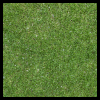
\includegraphics[scale=0.3]{GrassIcon}
	\end{minipage} \hfill
	\begin{minipage}{0.85\textwidth}
		Ikona typu dlaždic \texttt{Grass}, neboli tráva.
	\end{minipage}
}

\medskip
\noindent{
	\begin{minipage}{0.1\textwidth}
		
\includegraphics[scale=0.3]{WaterIcon}
	\end{minipage} \hfill
	\begin{minipage}{0.85\textwidth}
		Ikona typu dlaždic \texttt{Water}, neboli voda.
	\end{minipage}
}

\medskip
\noindent{
	\begin{minipage}{0.1\textwidth}
		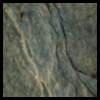
\includegraphics[scale=0.3]{StoneIcon}
	\end{minipage} \hfill
	\begin{minipage}{0.85\textwidth}
		Ikona typu dlaždic \texttt{Stone}, neboli kámen.
	\end{minipage}
}

\bigskip

Vybráním typu dlaždic z tohoto seznamu, umístěním kurzoru do herního světa a stisknutím levého tlačítka změníme typ dlaždic zvýrazněného čtverce na zvolený typ.

Pokud podržíme levé tlačítko a budeme pohybovat myší, budou změněny všechny dlaždice kterých se dotkně zvýrazněná část.

Velikost zvýrazněné části lze nastavit v okně nástrojů pomocí grafického prvku přidaného tímto nástrojem.

\subsubsection{Nástroj pro výběr a ovládání jednotek}
Tento nástroj umožňuje vybrat skupinu jednotek aktuálního hráče. Tento výběr uskutečníme stisknutím a držením levého tlačítka a následným tažením myši po herním světě. Mezi počáteční pozicí stisku a aktuální pozicí kurzoru se vytvoří obdélník označující oblast, ve které budou jednotky vybrány. Po uvolnění tlačítka myši budou všechny jednotky vlastněné aktuálním hráčem přidány do aktuálně vybrané skupiny jednotek. Jednotky lze označovat i jednotlivě kliknutím na jednotku vlastněnou aktuálním hráčem.

Následně lze vybraným jednotkám vydávat rozkazy. Kliknutím levým tlačítkem vydáme rozkaz k pohybu na aktuální pozici kurzoru. Kliknutím pravím tlačítkem na nepřátelskou jednotku či budovu pak vydáme rozkaz k útoku na tuto jednotku či budovu.

\subsubsection{Nástroj pro vytváření jednotek}
Tento nástroj umožňuje přidávat do aktuální úrovně nové jednotky či odebírat existující. Po zvolení tohoto nástroje je centrální lišta naplněna ikonami všech dostupných jednotek, které je možné manuálně přidávat do úrovně. Nejvíce vpravo je pak přidána ikona umožňující mazání existujících jednotek. V ukázkovém balíčku tedy bude centrální lišta vyplněna následujícími ikonami:

\medskip
\noindent{
	\begin{minipage}{0.1\textwidth}
		
\includegraphics[scale=0.3]{ChickenIcon}
	\end{minipage} \hfill
	\begin{minipage}{0.85\textwidth}
		Ikona typu jednotek \texttt{Chicken}.
	\end{minipage}
}

\medskip
\noindent{
	\begin{minipage}{0.1\textwidth}
		
\includegraphics[scale=0.3]{WolfIcon}
	\end{minipage} \hfill
	\begin{minipage}{0.85\textwidth}
		Ikona typu jednotek \texttt{Wolf}.
	\end{minipage}
}

\medskip
\noindent{
	\begin{minipage}{0.1\textwidth}
		
\includegraphics[scale=0.3]{Deleter}
	\end{minipage} \hfill
	\begin{minipage}{0.85\textwidth}
		Ikona pro odstraňování jednotek.
	\end{minipage}
}


\bigskip


Pro vytvoření nové jednotky vybereme jeden z poskytovaných typů a následným kliknutím do herního světa vytvoříme na pozici kurzoru novou jednotku vybraného typu.

Pro odstranění jednotky vybereme ikonu pro odstraňování jednotek. Následným kliknutím na jednotku tuto jednotku odstraníme z úrovně.

Funkcionalita tohoto nástroje je při hraní úrovně nahrazena budovou tvrze, popsanou v~části \ref{sec:buildings}.


\subsubsection{Nástroj pro stavbu budov}
\label{sec:buildingbuilder}
Tento nástroj umožňuje v editačním i v herním módu přidávat do herního světa budovy vlastněné aktuálně ovládaným hráčem. Při zvolení tohoto nástroje je centrální lišta vyplněna ikonami všech budov dostupných v balíčku. V ukázkovém balíčku bude centrální lišta vyplněna těmito ikonami:

\medskip
\noindent{
	\begin{minipage}{0.1\textwidth}
		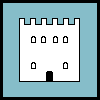
\includegraphics[scale=0.3]{KeepIcon}
	\end{minipage} \hfill
	\begin{minipage}{0.85\textwidth}
		Ikona typu budov \texttt{Keep}.
	\end{minipage}
}

\medskip
\noindent{
	\begin{minipage}{0.1\textwidth}
		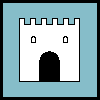
\includegraphics[scale=0.3]{GateIcon}
	\end{minipage} \hfill
	\begin{minipage}{0.85\textwidth}
		Ikona typu budov \texttt{Gate}.
	\end{minipage}
}

\medskip
\noindent{
	\begin{minipage}{0.1\textwidth}
		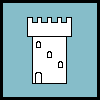
\includegraphics[scale=0.3]{TowerIcon}
	\end{minipage} \hfill
	\begin{minipage}{0.85\textwidth}
		Ikona typu budov \texttt{Tower}.
	\end{minipage}
}

\medskip
\noindent{
	\begin{minipage}{0.1\textwidth}
		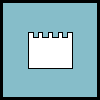
\includegraphics[scale=0.3]{WallIcon}
	\end{minipage} \hfill
	\begin{minipage}{0.85\textwidth}
		Ikona typu budov \texttt{Wall}.
	\end{minipage}
}

\medskip
\noindent{
	\begin{minipage}{0.1\textwidth}
		
\includegraphics[scale=0.3]{TreeCutterIcon}
	\end{minipage} \hfill
	\begin{minipage}{0.85\textwidth}
		Ikona typu budov \texttt{TreeCutter}.
	\end{minipage}
}

\medskip
\noindent{
	\begin{minipage}{0.1\textwidth}
		
\includegraphics[scale=0.3]{TreeIcon}
	\end{minipage} \hfill
	\begin{minipage}{0.85\textwidth}
		Ikona typu budov \texttt{Tree}.
	\end{minipage}
}

\medskip
\noindent{
	\begin{minipage}{0.1\textwidth}
		
\includegraphics[scale=0.3]{Deleter}
	\end{minipage} \hfill
	\begin{minipage}{0.85\textwidth}
		Ikona pro odstraňování budov.
	\end{minipage}
}

\bigskip

Následně vybráním jedné z těchto budov a kliknutím na dlaždici je do herního světa umístěna nová budova se středem na dané dlaždici. Tento nástroj dále umožňuje ovládání a mazání existujících budov. 

Ovládání je umožněno při aktivaci nástroje bez vybrané budovy, což následně umožňuje kliknutím na budovu zobrazit rozhraní pro její ovládání.

Mazání je umožněno výběrem ikony červeného čtverce a následným kliknutím na existující budovu.

\subsection{Ovládání kamery}
Kamera je schopna pohybu v~několika módech. Těmito módy jsou RTS mód, \texttt{FreeFloat} mód a~sledování jednotky. Přepínání mezi RTS a \texttt{FreeFloat} módem je prováděno klávesou \textit{Shift}. Přepnutí na sledování jednotky je možné kliknutím pravého tlačítka na jednotku. Následná lze přejít zpět na RTS mód pokusem o~pohnutí kamerou, či na \texttt{FreeFloat} mód pomocí klávesy \textit{Shift}.

Pohyb v~módech RTS a \texttt{FreeFloat} lze ovládat pomocí klávesnice. Klávesy \textit{W}, \textit{S}, \textit{A}, \textit{D} umožňují pohyb kamery vpřed, vzad, vlevo a~vpravo. 

V~módu RTS lze také ovládat pohyb kamery pomocí umístění myší na okraj obrazovky, načež se kamera začne posouvat směrem k~tomuto okraji. 

Otáčení kamery lze v~RTS módu a~módu sledování jednotky provést klávesami \textit{Q} a \texttt{E} pro otáčení vlevo či vpravo, a~klávesami \textit{R} a \textit{F} pro otáčení vzhůru a~dolu. 

V~módu \texttt{FreeFloat} lze otáčet kamerou pouze pomocí myši.   

\subsection{Budovy}
\label{sec:buildings}
Ukázkový balíček obsahuje šest typů budov. První čtyři typy označujeme jako obranné budovy, sloužící především pro zamezení průchodu nepřátelských jednotek a~umožňující zvýšení dostřelu vlastních jednotek pomocí umístění jednotek na tyto budovy. Mezi tyto budovy patří \texttt{Keep}, neboli tvrz, \texttt{Gate}, neboli brána, \texttt{Tower}, neboli věž a \texttt{Wall}, neboli hradba. Zbylé dva typy slouží pro získávání dřeva. Těmito budovami jsou \texttt{Tree}, neboli strom, a \texttt{TreeCutter}, neboli dřevorubec. 

\medskip
\noindent{
	\begin{minipage}{0.15\textwidth}
		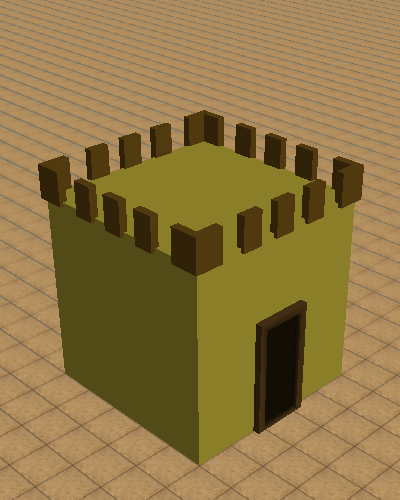
\includegraphics[scale=0.6]{Keep}
	\end{minipage} \hfill
	\begin{minipage}{0.8\textwidth}
		\textbf{Keep}, neboli tvrz. Každý hráč vlastní právě jednu tuto budovu, při jejímž zničení hráč prohrává. Cílem hry je tedy zničit protivníkovu tvrz bez ztráty své vlastní tvrze. Tvrz umožňuje pohyb jednotek po své střeše. Tvrz dále slouží pro tvorbu jednotek během hry. Tato funkce je zpřístupněna pomocí nástroje pro stavbu budov, popsaného v části \ref{sec:buildingbuilder}.
	\end{minipage}
}

\medskip
\noindent{
	\begin{minipage}{0.15\textwidth}
		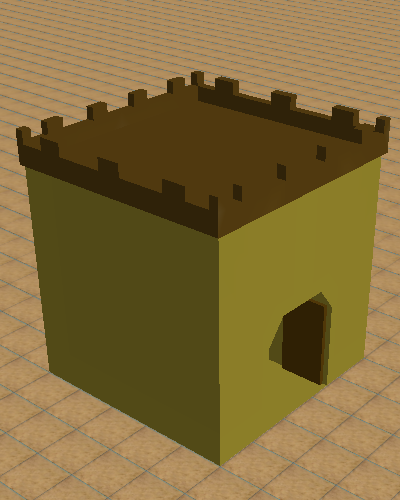
\includegraphics[scale=0.6]{Gate}
	\end{minipage} \hfill
	\begin{minipage}{0.8\textwidth}
		\textbf{Gate}, neboli brána. Brána umožňuje pohyb jednotek jak po své střeše, tak skrz tunel uvnitř této budovy. Střecha této budovy je automaticky propojena se střechami bran, věží a hradeb na přímo sousedících dlaždicích. Dále umožňuje již podle svého názvu zavřít jeden konec tunelu a~tím znemožnit přístup do tunelu z~této strany. Ovládání brány je zpřístupněno pomocí nástroje pro stavbu budov, popsaného v části \ref{sec:buildingbuilder}.
	\end{minipage}
}

\medskip
\noindent{
	\begin{minipage}{0.15\textwidth}
		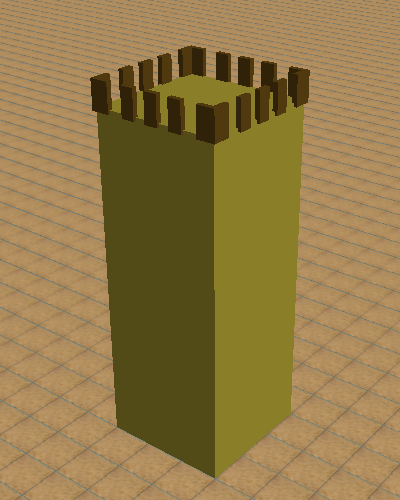
\includegraphics[scale=0.6]{Tower}
	\end{minipage} \hfill
	\begin{minipage}{0.8\textwidth}
		\textbf{Tower}, neboli věž. Tato budova umožňuje chůzi po své střeše a~díky své výšce zvyšuje dostřel jednotek. Její střecha je propojena se střechami bran, věží a hradeb na přímo sousedících dlaždicích.
	\end{minipage}
}

\medskip
\noindent{
	\begin{minipage}{0.15\textwidth}
		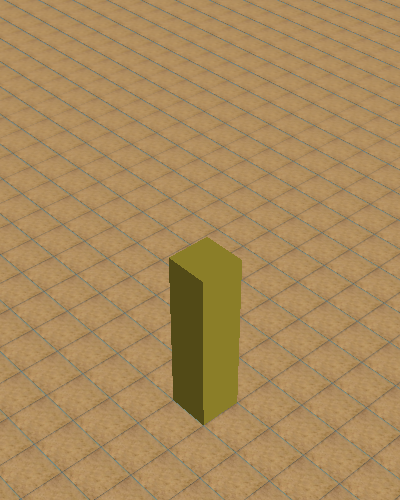
\includegraphics[scale=0.6]{Wall}
	\end{minipage} \hfill
	\begin{minipage}{0.8\textwidth}
		\textbf{Wall}, neboli hradba. Hlavním účelem této budovy je zablokování přístupu do hradu. Dále umožňuje chůzi po své střeše. Střecha je automaticky propojena se střechami bran, věží a hradeb přímo sousedících s touto budovou.
	\end{minipage}
}

\medskip
\noindent{
	\begin{minipage}{0.15\textwidth}
		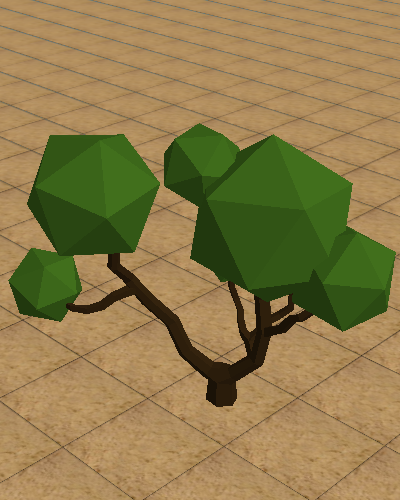
\includegraphics[scale=0.6]{Tree}
	\end{minipage} \hfill
	\begin{minipage}{0.8\textwidth}
		\textbf{Tree}, neboli strom. Stavba stromů je omezena na editaci úrovně a~jejich vlastníkem může být pouze neutrální hráč, tedy hráč s~šedým štítem. Tento hráč jako jediný nemusí vlastnit tvrz, nelze ho zabít a~neútočí na ostatní hráče. Stromy podle typu dlaždice, na které se nacházejí, rostou různou rychlostí a~množí se s~různou pravděpodobností.
	\end{minipage}
}

\medskip
\noindent{
	\begin{minipage}{0.15\textwidth}
		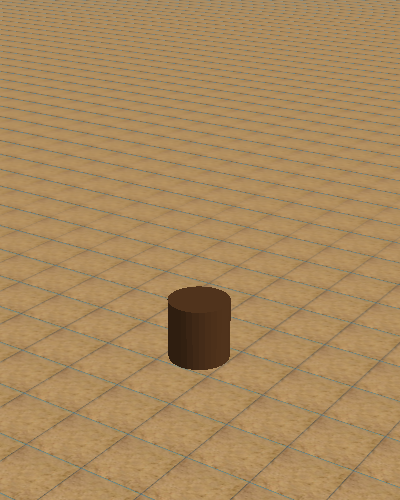
\includegraphics[scale=0.6]{TreeCutter}
	\end{minipage} \hfill
	\begin{minipage}{0.8\textwidth}
		\texttt{TreeCutter}, neboli dřevorubec umožňuje hráči získávat ze stromů dřevo. Tato budova vytváří dvě jednotky, které následně pendlují mezi nejbližším stromem a~touto budovou, čímž získávají pro hráče dřevo.
	\end{minipage}
}

\subsection{Jednotky}
Balíček ukázkové hry definuje tři typy jednotek, z toho dvě ovladatelné hráčem a jednu plně automatickou.

\medskip
\noindent{
	\begin{minipage}{0.15\textwidth}
		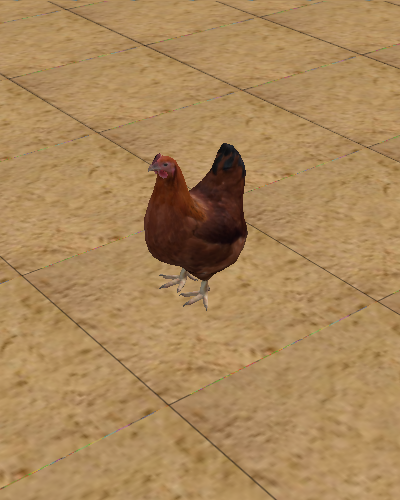
\includegraphics[scale=0.6]{Chicken}
	\end{minipage} \hfill
	\begin{minipage}{0.8\textwidth}
		\textbf{Chicken} je jednotka útočící na dálku, používající vajíčka jako projektily. Dostřel této jednotky závisí na rozdílu její výšky od cíle, je tedy výhodné ji umisťovat na vyvýšená místa, jako například budovy. Oproti vlkům dokáže tento typ jednotek chodit přes vodu a~poškodit obranné budovy.
	\end{minipage}
}

\medskip
\noindent{
	\begin{minipage}{0.15\textwidth}
		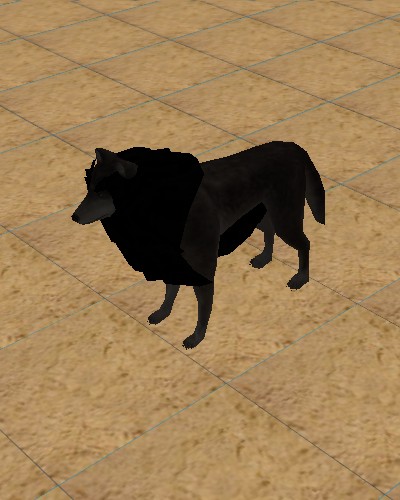
\includegraphics[scale=0.6]{Wolf}
	\end{minipage} \hfill
	\begin{minipage}{0.8\textwidth}
		\textbf{Wolf}, neboli vlk, je jednotka útočící na blízko. Tato jednotka se pohybuje rychleji než \texttt{Chicken} nebo \texttt{Dog}. Tato jednotka nedokáže poškodit nepřátelské obranné budovy.
	\end{minipage}
}

\medskip
\noindent{
	\begin{minipage}{0.15\textwidth}
		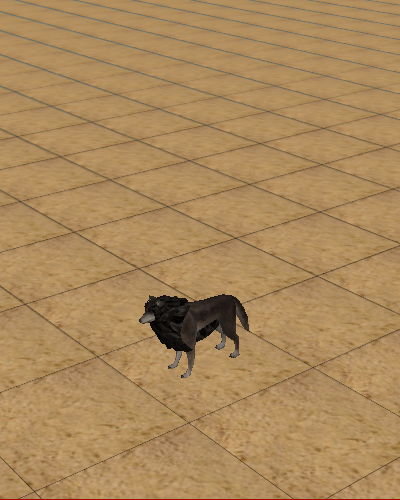
\includegraphics[scale=0.6]{Dog}
	\end{minipage} \hfill
	\begin{minipage}{0.8\textwidth}
		\textbf{Dog}, neboli pes, je jednotka vytvářená budovou dřevorubce, která se pohybuje mezi budovou a nejbližším stromem a získává tak dřevo. Tuto jednotku nelze manuálně vytvářet ani ovládat, vše je plně automatizováno. 
	\end{minipage}
}

\subsection{Projektily}
Ukázková hra definuje pouze jeden projektilů, ze kterých je pouze jeden aktuálně využíván. Těmito typy jsou:

\begin{enumerate}
	\item \texttt{EggProjectile},
	\item \texttt{TestProjectile}.
\end{enumerate}

První typ je využíván jednotkou \texttt{Chicken}. Tento typ má jednoduchou logiku využívající komponenty \texttt{BallisticProjectile} pro implementaci svého pohybu. Drhý typ ukazuje možnosti složitějšího chování projektilu. Tento projektil také využívá pro implementaci svého pohybu komponentu \texttt{BallisticProjectile}, ale dále přidává dodatečné chování. Po určité době od výstřelu se tento projektil rozdělí na více projektilů stejného druhu, čímž vytvoří efekt brokovnice a~pokryje projektily okolí svého původního dopadu. Dále tento projektil ukazuje zpožděné odstranění z~úrovně, díky kterému zůstává určitou chvíli zaseknutý v~terénu.

\subsection{Umělé inteligence hráčů}
Ukázková hra poskytuje dvě umělé inteligence nepřátelských hráčů, kterými jsou:

\begin{enumerate}
	\item \texttt{LazyPlayer},
	\item \texttt{AggressivePlayer}.
\end{enumerate}

Lazy player je jednoduchá umělá inteligence, která nic nedělá. Jejím hlavním účelem umožnění uživately vyzkoušení herního režimu platformy a~možnost stavby svého hradu bez jakéhokoli ohrožení nepřítelem.

AggressivePlayer je aktivní umělá inteligence, která staví budovy pro získávání dřeva, jednotky pro obranu svého tvrze a~útok na nejbližšího nepřátelského hráče.

\subsection{Umělé inteligence úrovní}
Ukázková hra je příkladem balíčku, který všechnu svou logiku decentralizuje do jednotek, budov, projektilů a~hráčů. Z~tohoto důvodu obsahují dvě logiky definované ukázkovou hrou minimum herní logiky. Ukázková hra poskytuje tyto dvě logiky:

\begin{enumerate}
	\item \texttt{TwoPlayerLogic},
	\item \texttt{FourPlayerLogic}.
\end{enumerate}

Obě tyto logiky poskytují požadované metody informace platformě ve formě \texttt{ToolManageru} a \texttt{AStarFactory}. 

První logika již podle názvu definuje úrovně se dvěma hráči. Dále poskytuje možnost před prvním spuštěním úrovně nastavit počáteční množství surovin vlastněné hráči.
Druhá logiky definuje úrovně se čtyřmi hráči a~určuje pevné množství počátečních surovin.
